\documentclass[cs4size,a4paper,nofonts]{ctexart}
\usepackage[utf8]{inputenc}
\def\tjf{{\tt{田劲锋}}}
\def\titlec{企业应用集成系统}
\def\version{V0.0.3}
\usepackage[b5paper,margin=2cm]{geometry} % 页面设置
\usepackage[unicode,breaklinks=true,
colorlinks=true,linkcolor=black,anchorcolor=black,citecolor=black,urlcolor=black,
pdftitle={\titlec \version},pdfauthor={\tjf}]{hyperref}
%\CTEXsetup[number=\chinese{section}, format={\large\sf\bfseries}]{section}
\usepackage{latexsym,amsmath,amssymb,bm}

\setmainfont{Times New Roman}
\setCJKmainfont[BoldFont={SimHei}]{SimSun}  % 主要字体:宋体、黑体
\setCJKsansfont[BoldFont={STZhongsong}]{STFangsong} % 次要字体:仿宋、中宋
\setCJKmonofont{KFKai} % 等宽字体:楷体

\CJKsetecglue{\hspace{0.1em}}
\renewcommand\CJKglue{\hskip -0.3pt plus 0.08\baselineskip}
\frenchspacing
\widowpenalty=10000
\linespread{1.2} % 行距

\usepackage[inline]{enumitem} % 调整列表样式
\setlist{noitemsep}
\setlist[itemize]{topsep=0pt,partopsep=0pt,itemsep=0pt,parsep=0pt}
\setlist[enumerate]{topsep=0pt,partopsep=0pt,itemsep=0pt,parsep=0pt,label={\arabic{section}.\arabic{subsection}.\arabic*}}
\setlist[enumerate,2]{label*={.\arabic*}}

%\makeindex
\pagestyle{plain}

\begin{document}

%%%% 开始 %%%%

\title{\bf\titlec~\version}
\author{软件工程1305班~\quad\tjf\quad~201316920311}
\maketitle

\section{业务需求}

企业应用集成(Enterprise Application Integration, EAI)是一个或多个系统的集合,并使两个以上的后台应用能够作特定数据的统一管理系统,并能保证这些后台应用同步良好。这样的系统可以为单个公司提供其所有信息的集中访问点。

通过应用集成,提高业务流程的自动化程度,获得如下好处:

\begin{itemize}
\item 增强业务处理的可靠性
\item 缩短处理时间
\item 减少人工干涉
\item 保证数据一致性
\item 获得更高质量的报表数据
\item 降低运营成本
\end{itemize}

本系统将来进行可以通过插件方式进行扩展,组合成功能全面的企业资源计划(Enterprise Resource Planning, ERP)系统。

\section{用户需求}

对于小型中型的商业公司,通常会使用多个软件系统来处理不同的事务。用户手工操作资金结算系统、发票管理系统、销售管理系统、客户服务系统,其数据都是手工完成输入的,工作时要打开多个软件,在不同的窗口之间复制、粘贴,甚至使用电子表格来处理软件系统没有提供的功能。

用户需要一个集成平台系统,尽可能来整合这些软件系统,从而减轻工作量,减少错误发生。

系统需要支持这些功能:

\begin{itemize}
\item 追踪单个请求处理状态
\item 保存用户请求日志
\item 生成各种审计报告
\item 保存系统响应日志
\item 以同步或异步的方式处理请求
\item 回滚处理流程机制
\item 搜索条目和内容
\item 事务中断处理
\item 提供统一用户界面
\end{itemize}

%假设现有的系统有:

%\paragraph{结算系统}

%\paragraph{销售管理系统}

%\paragraph{客户服务系统}

\subsection{功能需求}

\begin{enumerate}
\item 【平台通用】
系统处理来自各方的请求,该机制不会限制用户或其他系统,也不限制开发环境、编程语言和操作系统。
\item 【调用接口】
系统提供一个不依赖于环境的交互接口,使用机器和人皆可读的 XML 或者 JSON 格式可以提供一个这样的中间平台。
\item 【日志记录】
要求详细记录经过系统产生的一切处理过程,包括但不限于这些信息:编号、处理情况、提交和解决时间、处理方案和步骤。
\item 【日志查询】
提供查询记录日志的功能,用户可以按关键字查询、排序以及按条件查询。
\item 【用户验证】
提供用户注册和登录功能,为每个用户产生其需要的数据和界面。
\item 【用户权限】
为不同的用户分配不同的权限和角色,保障系统安全性和业务稳定性。用户权限设置要灵活,然而根用户例外。
\item 【用户锁定】
对于多次执行了非法操作的用户,如多次输错密码,系统将自动锁定用户一定时间,并有管理员决策是否解除锁定。
\item 【集成扩展】
系统要可以实现新增功能和业务流程的插入和修改功能,实现集成系统的扩展,以便适应用户不断变化的业务需求。
\item 【业务组合】
系统将多项任务组合成单个逻辑的用户请求,通过把若干相关的处理过程整合成为一个请求,用户可以将一系列相关操作组合成逻辑上的统一整体,并包含在单个请求中进行处理。
\item 【输入验证】
系统要验证数据输入的合法性,这是保证系统能够正常运行的必要条件。通过操作进行之前的输入验证和修正,可以预防后期修正导致的一连串棘手问题。
\item 【业务处理】
需要在请求处理过程中落实业务规则,验证用户通用的要求和自定义要求,根据不同情况处理状态和数据库,在此基础上制作数据报表和性能报表。
\item 【请求回滚】
对于包含多个步骤的处理请求,有些可以容忍的错误可以记录在日志中,有些错误不可容忍,需要中止整个请求的处理,甚至需要恢复请求之前的数据系统状态。
\item 【管理报告】
日志查询的升级版,提供图表形式的日志数据。通过对日志数据的分析,系统生成不同种类的报告提供给系统管理员分析和检查问题。
\item 【实时警报】
对于严重的系统错误,影响到了用户利益,应当提供途径向相关人员发送警报信息,以便进一步处理。方式包括但不限于电子邮件、手机短信、即时通讯等。
\item 【灾难恢复】
当系统运转过程中产生了不可避免的意外事故,如断电等,将导致处理结果不完整。有必要在分解请求的基础上,及时保存请求处理到数据库中,同时提供措施以便恢复用户提交而未能及时处理的任务。

\end{enumerate}

\section{需求建模}

图~\ref{dfd0}~描述了系统最顶层的数据流。Web 服务器从用户处接收业务处理请求的消息,在记录如数据库的同时将组合业务逻辑转发给 EAI 后台,后台将业务分解到各个子系统中,并记录数据库。

\begin{figure}[htp]
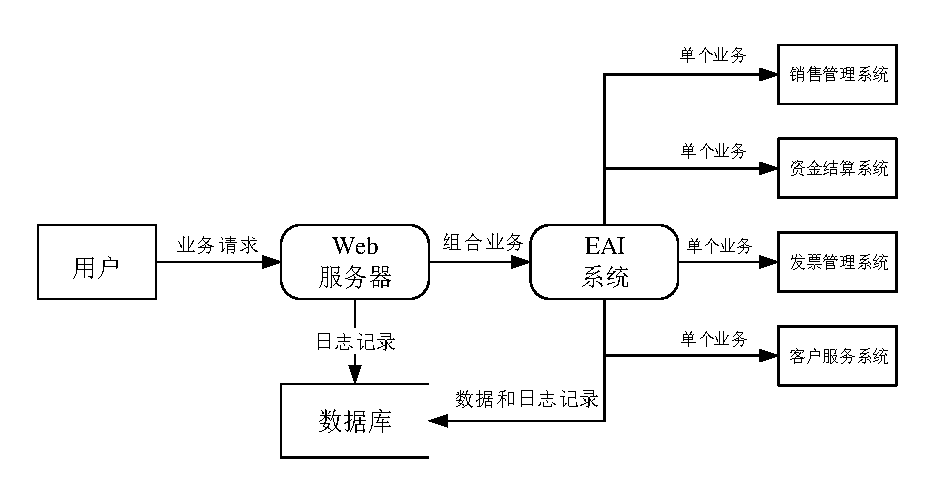
\includegraphics[width=\textwidth,page=1]{images/dfd.pdf}
\caption{\label{dfd0}系统顶级数据流图}
\end{figure}

顶级数据流包含两个主要的处理逻辑,这里将其描述为一级数据流图。

图~\ref{dfd1.1}~描述了用户请求的数据流程,也就是 Web 服务器的处理流程。

\begin{figure}[htp]
\includegraphics[width=\textwidth,page=2]{images/dfd.pdf}
\caption{\label{dfd1.1}一级数据流图:用户请求的处理}
\end{figure}

图~\ref{dfd1.2}~描述了 EAI 系统的后端处理的数据流程。

\begin{figure}[htp]
\includegraphics[width=\textwidth,page=3]{images/dfd.pdf}
\caption{\label{dfd1.2}一级数据流图:EAI 系统的后端处理}
\end{figure}

\end{document}
